\documentclass[border=8pt]{standalone}
\usepackage{amsmath,amssymb}
\usepackage{tikz}
\usetikzlibrary{arrows.meta, positioning}
\begin{document}
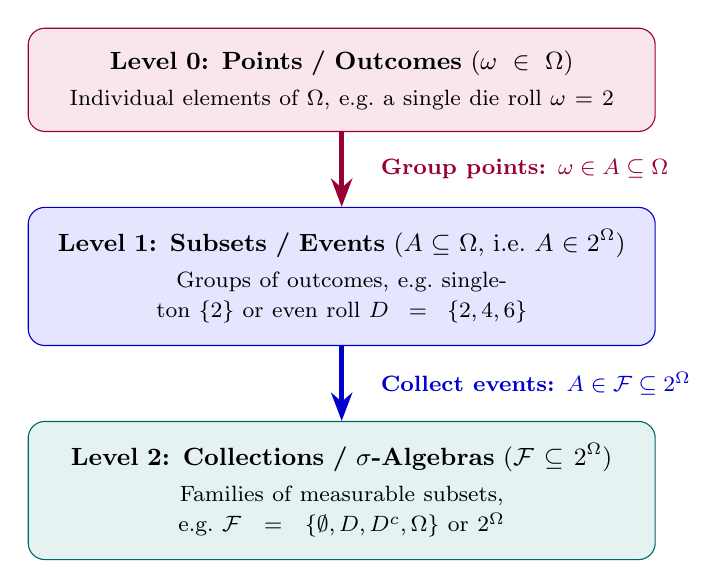
\begin{tikzpicture}[font=\small, >=Stealth]
  \node[draw=purple!80!black, rounded corners=6pt, fill=purple!10, text width=7.4cm, align=center, inner sep=8pt] (L0)
    {\textbf{Level 0: Points / Outcomes} ($\omega \in \Omega$) \\[2pt]
     \footnotesize Individual elements of $\Omega$, e.g.\ a single die roll $\omega = 2$};

  \node[draw=blue!80!black, rounded corners=6pt, fill=blue!10, text width=7.4cm, align=center, inner sep=8pt, below=0.95cm of L0] (L1)
    {\textbf{Level 1: Subsets / Events} ($A \subseteq \Omega$, i.e.\ $A \in 2^\Omega$) \\[2pt]
     \footnotesize Groups of outcomes, e.g.\ singleton $\{2\}$ or even roll $D = \{2, 4, 6\}$};

  \node[draw=teal!80!black, rounded corners=6pt, fill=teal!10, text width=7.4cm, align=center, inner sep=8pt, below=0.95cm of L1] (L2)
    {\textbf{Level 2: Collections / $\sigma$-Algebras} ($\mathcal{F} \subseteq 2^\Omega$) \\[2pt]
     \footnotesize Families of measurable subsets, e.g.\ $\mathcal{F} = \{\emptyset, D, D^c, \Omega\}$ or $2^\Omega$};

  \draw[->, line width=1.6pt, purple!80!black] (L0) -- (L1)
    node[midway, right=10pt, font=\footnotesize\bfseries, text=purple!80!black] {Group points: $\omega \in A \subseteq \Omega$};
  \draw[->, line width=1.6pt, blue!80!black] (L1) -- (L2)
    node[midway, right=10pt, font=\footnotesize\bfseries, text=blue!80!black] {Collect events: $A \in \mathcal{F} \subseteq 2^\Omega$};
\end{tikzpicture}
\end{document}
